
%(BEGIN_QUESTION)
% Copyright 2006, Tony R. Kuphaldt, released under the Creative Commons Attribution License (v 1.0)
% This means you may do almost anything with this work of mine, so long as you give me proper credit

This {\it chromatogram} shows the separation of five different substances over time:

$$\includegraphics[width=15.5cm]{i00672x01.eps}$$

Note how components 4 and 5 are not clearly differentiated in the chromatogram.  Identify at least one way the chromatograph could be altered to obtain clearer separation (better {\it resolution}) of these last two components.

\underbar{file i00672}
%(END_QUESTION)





%(BEGIN_ANSWER)

\begin{itemize}
\item{} Use a denser stationary phase in the column.
\item{} Use a stationary phase with better adsorptivity (and/or solubility).
\item{} Use temperature or flow ``programming'' to slow down the elution of that last two components to achieve better separation
\end{itemize}

%(END_ANSWER)





%(BEGIN_NOTES)


%INDEX% Measurement, analytical: chromatography

%(END_NOTES)


